% !TeX spellcheck = fr_FR

% TODO: Replace scan images with clean text where possible

\documentclass[a4paper, 10pt]{report}

\usepackage[french]{babel}
\usepackage[T1]{fontenc}

\usepackage{amsmath, amssymb, amsfonts}

\usepackage{hyperref}
\usepackage{geometry}

\usepackage{xcolor}
\usepackage{graphicx}

\usepackage{fancyhdr}
\usepackage{lastpage}

\usepackage{enumitem}

\geometry{
	a4paper,
	left=25mm,
	right=25mm,
	top=35mm,
	bottom=25mm,
	headsep=5mm,
	headheight=20mm,
}

\definecolor{solution}{HTML}{E5E4E2}
\providecommand{\abs}[1]{\lvert#1\rvert}
\providecommand{\norm}[1]{\lVert#1\rVert}
\DeclareMathOperator{\card}{card}

\begin{document}
	
	\renewcommand{\headrule}{%
		\vspace{-4pt}\hrulefill
		\raisebox{-6.8pt}{\ 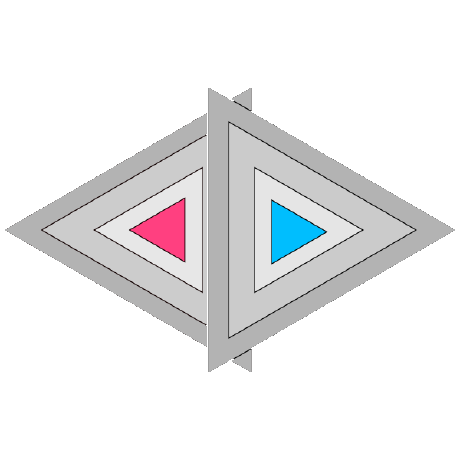
\includegraphics[height=5mm]{../../icon.png}}
		\hrulefill
	}	
	\pagestyle{fancy}
	\fancyhf{}
	
	\fancyhead[L]{\small \slshape Automne 2024}
	\fancyhead[C]{\Large \bfseries Algèbre I - Série 04}
	\fancyhead[R]{\small Buff Mathias}
	\fancyfoot[L]{
		\small Source files available at:
		\href{https://github.com/MathiasBuff/bsc-math}
		{github.com/MathiasBuff/bsc-math}
	}
	\fancyfoot[R]{
		\small Page \thepage
		\hspace{1pt} /
		\pageref*{LastPage}
	}
	

	\noindent
	\textbf{Exercice 1.} (Compléter une famille libre en une base)\\
	Considérons l'ensemble suivant de matrices :
	\[
		\mathcal{F} = \left\{
			\begin{pmatrix}
				0& 1\\
				0& 1
			\end{pmatrix},
			\begin{pmatrix}
				1& 0\\
				1& 0
			\end{pmatrix},
			\begin{pmatrix}
				\phantom{-}1& -1\\
				-1& \phantom{-}1
			\end{pmatrix}
			\right\}
	\]
	
	\begin{enumerate}[label=\arabic*.]
		\item Montrer que $\mathcal{F}$ est une famille libre de
		$\mathcal{M}_{2, 2}(\mathbb{R})$ (sur $\mathbb{R}$).
		%
		\item Compléter $\mathcal{F}$ en une base de
		$\mathcal{M}_{2, 2}(\mathbb{R})$ (sur $\mathbb{R}$).
		Justifier votre réponse.
	\end{enumerate}
	
	\colorbox{solution}
	{
		\begin{minipage}{0.9\textwidth}
			\begin{enumerate}[label=\arabic*.]
				\item $\lambda_1 \cdot \begin{pmatrix}0&1\\0&1\end{pmatrix}
				+ \lambda_2 \cdot \begin{pmatrix}1&0\\1&0\end{pmatrix}
				+ \lambda_3 \cdot \begin{pmatrix}1&-1\\-1&1\end{pmatrix}
				= \begin{pmatrix}
					\lambda_2 + \lambda_3 & \lambda_1 - \lambda_3\\
					\lambda_2 - \lambda_3 & \lambda_1 + \lambda_3
				\end{pmatrix}$
				avec $\lambda_1, \lambda_2, \lambda_3 \in \mathbb{R}$
				\vspace{6pt}
				
				et
				$\left\{\begin{matrix}
					\lambda_2 + \lambda_3 = 0 \\
					\lambda_1 - \lambda_3 = 0 \\
					\lambda_2 - \lambda_3 = 0 \\
					\lambda_1 + \lambda_3 = 0
				\end{matrix}\right.
				\qquad
				\left\{\begin{matrix}
					2\lambda_3 = 0 \\
					\lambda_1 = \lambda_3 \\
					\lambda_2 = \lambda_3 \\
					2\lambda_3 = 0
				\end{matrix}\right.
				\qquad
				\lambda_1 = \lambda_2 = \lambda_3 = 0$\\
				
				Donc, $\mathcal{F}$ est libre.
				
				\vspace{12pt}
				\item Puisque $\dim \mathcal{M}_{2,2}(\mathbb{R}) = 4$
				et $\abs{\mathcal{F}} = 3$, il faut ajouter un vecteur
				à $\mathcal{F}$ pour la compléter en une base de
				$\mathcal{M}_{2,2}(\mathbb{R})$.\vspace{6pt}
				
				Par le lemme d'échange, on peut trouver un vecteur parmi
				la base canonique de $\mathcal{M}_{2,2}(\mathbb{R})$
				qui satisfait nos conditions.\vspace{6pt}
				
				Par exemple, $\left(\begin{smallmatrix}
						0&0\\0&1\end{smallmatrix}\right)$
				n'est pas exprimable comme combinaison linéaire des
				vecteurs de $\mathcal{F}$, donc $\mathcal{F} \cup
					\left\{\left(\begin{smallmatrix}0&0\\0&1
					\end{smallmatrix}\right)\right\}$
				est libre, et comme elle possède 4 éléments, c'est une
				base de $\mathcal{M}_{2,2}(\mathbb{R})$ sur $\mathbb{R}$.
			\end{enumerate}
		\end{minipage}
	}
	
	\vspace{5mm}
	\noindent
	\textbf{Exercice 2.} (Compléter un sous-espace vectoriel)\\
	Considérons le sous-espace vectoriel
	$W = \{p(x) = a_0 + a_1x + a_2x^2 + a_3x^3 \mid p(1) = 0\}
		\subset \mathbb{R}_3[x]$ sur $\mathbb{R}$.
	
	\begin{enumerate}[label=\arabic*.]
		\item Trouver une base de $W$ et en déduire sa dimension.
		%
		\item Trouver un sous-espace $V \subset \mathbb{R}_3[x]$ tel que
		$\mathbb{R}_3[x] = W \oplus V$.
	\end{enumerate}
	
	\colorbox{solution}
	{
	\begin{minipage}{0.9\textwidth}
		\begin{enumerate}[label=\arabic*.]
			\item Puisque $p(1) = 0$, alors $a_0 + a_1 + a_2 + a_3 = 0$.
			Par conséquent, $W$ peut être généré en laissant
			$a_1x, a_2x^2, a_3x^3$ libres, et en contraignant $a_0$ par
			$a_0 = -a_1 - a_2 - a_3$.
			
			Ainsi, $\{(-1 + x), (-1 + x^2), (-1 + x^3)\}$ est une base
			de $W$, donc $\dim W = 3$.
			
			\vspace{12pt}
			\item $\dim \mathbb{R}_3[x] = \dim W + \dim V$, donc
			$\dim V = \dim \mathbb{R}_3[x] - \dim W = 1$. Par
			conséquent, nous devons trouver un vecteur de $\mathbb{R}_3[x]$
			qui n'est pas contenu dans $W$, et ce vecteur suffira pour
			former une base de $V$.\vspace{6pt}
			
			Par exemple, $p = (1) = (1 + 0x + 0x^2 + 0x^3)$ n'est pas
			contenu dans $W$, car $p(1) = 1 \neq 0$.
			Donc, $\{(1)\}$ est une base de $V$ qui satisfait
			$\mathbb{R}_3[x] = W \oplus V$.\\
			(On remarquera que ce choix donne $V = \mathbb{R}_0[x]$).
		\end{enumerate}
	\end{minipage}
	}
	
	\newpage
	
	\fancyhf{}
	\renewcommand{\headrule}
	{\rule{\textwidth}{0pt}}
	\fancyfoot[R]{
		\small Page \thepage
		\hspace{1pt} /
		\pageref*{LastPage}
	}
	
	\noindent
	\textbf{Exercice 3.} (Somme, intersection et dimension de sous-espaces)\\
	
	\begin{enumerate}[label=\arabic*.]
		\item Soient $F, G, H$ trois sous-espaces vectoriels d'un espace
		vectoriel $E$. Les inclusions suivantes sont-elles vraies ?
		Le prouver ou donner un contre-exemple.
		\begin{gather*}
			F \cap (G + H) \subset F \cap G + F \cap H \\
			F \cap G + F \cap H \subset F \cap (G + H)
		\end{gather*}
		
		\colorbox{solution}
		{
			\begin{minipage}{0.9\textwidth}
				$F \cap (G + H) \subset F \cap G + F \cap H$ est FAUSSE.\\
				\underline{Preuve par contre-exemple} :\textit{(avec
					$\{e_1, e_2, e_3\}$ la base canonique de
					$\mathbb{R}^3$)}\vspace{6pt}
				
				Soit $F = \langle\{e_1, e_2\}\rangle,
					G = \langle\{e_2, e_3\}\rangle
					H = \langle\{e_1, e_3\}\rangle$. Alors,\\
				$F \cap (G + H) = \langle\{e_1, e_2\}\rangle \cap
					\big(\langle\{e_2, e_3\}\rangle +
						\langle\{e_1, e_3\}\rangle\big)
					= \langle\{e_1, e_2\}\rangle \cap 
					\langle\{e_1, e_2, e_3\}\rangle
					= \langle\{e_1, e_2, e_3\}\rangle$\\
				et $F \cap G + F \cap H
					= \langle\{e_1, e_2\}\rangle \cap
					\langle\{e_2, e_3\}\rangle
					+ \langle\{e_1, e_2\}\rangle \cap
					\langle\{e_1, e_3\}\rangle
					= \langle\{e_2\}\rangle + \langle\{e_1\}\rangle
					=\langle\{e_1, e_2\}\rangle$\vspace{6pt}
				
				Donc, $e_3 = (0,0,1) \in F \cap (G + H)$ mais
				$e_3 \not\in F \cap G + F \cap H$, donc
				$F \cap (G + H) \not\subset F \cap G + F \cap H$.\vspace{12pt}
				
				$F \cap G + F \cap H \subset F \cap (G + H)$ est VRAIE.\\
				\underline{Preuve :}\vspace{6pt}
				
				Soit $v \in F \cap G + F \cap H, i.e.\
					v = \sum_{i \in I}g_i + \sum_{j \in J}h_j$,
				où $g_i$ est un vecteur d'une base de $F \cap G$ et
				$h_j$ est un vecteur d'une base de $F \cap H$.\\
				En particulier : \begin{itemize}
					\item $g_i$ et $h_j \in F$, donc $v \in F$
					\item $g_i \in G$ et $h_j \in H$, donc $v \in G + H$
				\end{itemize}
				Donc, $v \in  F \cap (G + H)$.
			\end{minipage}
		}
		%
		\item Soient $U$ et $V$ deux sous-espaces de $\mathbb{R}^6$
		tels que $\dim(U) = 2$ et $\dim(V) = 5$.
		\begin{enumerate}[label=(\alph*)]
			\item Quelles sont les valeurs minimales et maximales de
			$\dim(U + V)$ ? Donner des exemples concrets.
			\item Quelles sont les valeurs minimales et maximales de
			$\dim(U \cap V)$ ? Donner des exemples concrets.
		\end{enumerate}
		
		\colorbox{solution}
		{
			\begin{minipage}{0.9\textwidth}
				\begin{enumerate}[label=(\alph*)]
					\item Si $U \subset V$, par exemple
					$U = \langle\{e_1, e_2\}\rangle$ et
					$V = \langle\{e_1, e_2, e_3, e_4, e_5\}\rangle$\\
					\textit{(où $\{e_1, e_2, e_3, e_4, e_5, e_6\}$
					est la base canonique de $\mathbb{R}^6$)}\\
					Alors $U + V = V$ et $\dim(U + V) = \dim(V) = 5$.
					\vspace{6pt}
					
					Sinon, par exemple $U = \langle\{e_1, e_2\}\rangle$
					et $V = \langle\{e_2, e_3, e_4, e_5, e_6\}\rangle$\\
					Alors $U + V = \mathbb{R}^6$ et $\dim(U + V)
						= \dim(\mathbb{R}^6) = 6$.
					
					\vspace{12pt}
					\item En reprenant les mêmes exemples que pour (a),
					on a $1 \leq \dim(U \cap V) \leq 2$.
				\end{enumerate}
			\end{minipage}
		}
		%
		\item Considérons les sous-espaces de $\mathbb{R}^4$ suivants
		\begin{gather*}
			U = \{
				(x, y, z, t) \in \mathbb{R}^4 \mid 2x + 3z - 4t = 0\
				\text{et}\ 3z -2t = 0
				\} \\
			W = \Big\langle\{
				(1, 0, 0, 0),\ (0, 4, 0, 0),\ (2, -1, 0, 0),\ (0,0,0,1)
				\}\Big\rangle
		\end{gather*}
		\begin{enumerate}[label=(\alph*)]
			\item Calculer la dimension de $U$ et de $W$.
			\item Montrer que $U + W = \mathbb{R}^4$
		\end{enumerate}
		
		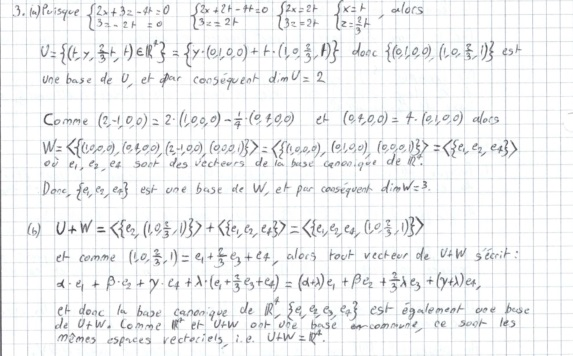
\includegraphics[scale=0.8]{ex03-p3.jpg}
	\end{enumerate}
	
	
	
	\vspace{5mm}
	\noindent
	\textbf{Exercice 4.} (Matrices symétriques et antisymétriques)\\
	Soit $\mathcal{M}_{n, n}(\mathbb{R})$ l'espace vectoriel des matrices
	carrées sur $\mathbb{R}$ de taille $n$. La transposée de la matrice
	$A = (a_{ij})_{i, j = 1, \dotsc, n}$ est définie comme
	$A^{\top} = (a_{ji})_{i, j = 1, \dotsc, n}$ (\textit{i.e.} on échange
	les lignes avec les colonnes).\\
	
	\textbf{Partie A -} Soit $\mathcal{S}_n(\mathbb{R})
		= \{A \in \mathcal{M}_{n, n}(\mathbb{R}) \mid A = A^{\top}\}$
	l'ensemble des matrices \textit{symétriques}.
	\begin{enumerate}[label=\arabic*.]
		\item Montrer que $\mathcal{S}_n(\mathbb{R})$ est un sous-espace
		vectoriel de $\mathcal{M}_{n, n}(\mathbb{R})$
		%
		\item Donner une base de $\mathcal{S}_n(\mathbb{R})$ dans le cas
		où $n = 3$
		%
		\item Quelle est la dimension de $\mathcal{S}_n(\mathbb{R})$?
		\\
	\end{enumerate}
	
	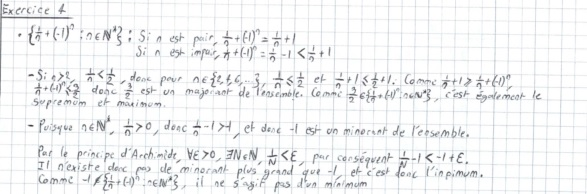
\includegraphics[scale=0.8]{ex04-p1.jpg}
	
	\textbf{Partie B -} Soit $\mathcal{A}_n(\mathbb{R})
	= \{A \in \mathcal{M}_{n, n}(\mathbb{R}) \mid A = -A^{\top}\}$
	l'ensemble des matrices \textit{antisymétriques}.
	\begin{enumerate}[label=\arabic*.]
		\item Montrer que $\mathcal{A}_n(\mathbb{R})$ est un sous-espace
		vectoriel de $\mathcal{M}_{n, n}(\mathbb{R})$
		%
		\item Donner une base de $\mathcal{A}_n(\mathbb{R})$ dans le cas
		où $n = 3$
		%
		\item Quelle est la dimension de $\mathcal{A}_n(\mathbb{R})$?
		\\
	\end{enumerate}
	
	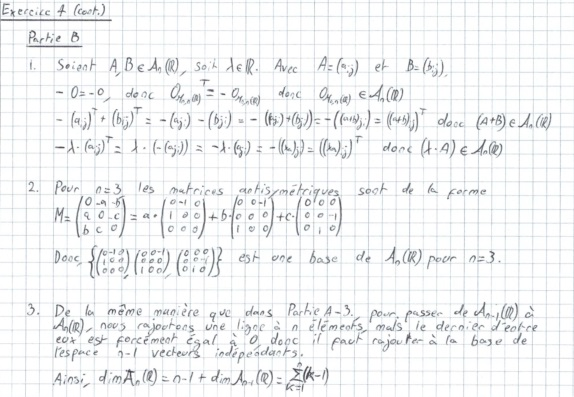
\includegraphics[scale=0.8]{ex04-p2.jpg}
		
	\textbf{Partie C}
	\begin{enumerate}[label=\arabic*.]
		\item Décrire explicitement les ensembles
		\[
			\mathcal{S}_n(\mathbb{R}) + \mathcal{A}_n(\mathbb{R}),
			\quad
			\mathcal{S}_n(\mathbb{R}) \cap \mathcal{A}_n(\mathbb{R})
		\]
		Que peut-on en conclure ?
		%
		\item En argumentant sur les dimensions, vérifier l'égalité
		$\mathcal{M}_{n, n}(\mathbb{R}) =
			\mathcal{S}_n(\mathbb{R}) \oplus \mathcal{A}_n(\mathbb{R})$
	\end{enumerate}
	
	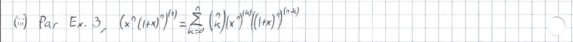
\includegraphics[scale=0.8]{ex04-p3.jpg}	
	
%	
%	\colorbox{solution}
%	{
%		\begin{minipage}{0.9\textwidth}
%			s
%		\end{minipage}
%	}
%	
%	\colorbox{solution}
%	{
%		\begin{minipage}{0.9\textwidth}
%			\begin{enumerate}[label=(\alph*)]
%				\item a
%			\end{enumerate}
%		\end{minipage}
%	}
	
\end{document}
